\chapter[Lecture 4]{}\label{lec4}

\section*{Group Theory and Qu.Mech.}

\subsection*{Group}

Group is a set of elements $A$, $B$, $C$ such that a for an of operation may be defined between two elements creating a third element
\begin{center}
operation $\to$ group multiplication
\end{center}
The above operation must satisfy the following criteria.
\begin{itemize}
\item[(i)] Closure property : The product of any two element is in the set. $AB=C$ all are elements of the group.

\item[(ii)] Associative law : $A(BC)=(AB)C$

\item[(iii)] There is a unit element : $E\Rightarrow EA=AE=A$

\item[(iv)] There exist an inverse to each element.
$$
A^{-1}:AA^{-1}=A^{-1}A=E
$$
\end{itemize}
For our use, we restrict to finite group $\to$ No. of elements, $h$ is finite.

$\to$ $h$ is called the order of the group.

\subsection*{Abelian}

If the group multiplication is {\bf commutative}, it is called {\bf abelian group.}

\section*{Example}

\noindent
{\bf Abelian group:} Set of all (+ve) and (-ve) integers including `0' $\to$ natural numbers, here inverse is defined as changing sing unit is `0' and group multiplication operation $\to$ addition.

\noindent
{\bf Non-abelian group:} Set of $n\times n$ matrices having non-zero determinants.

group multiplication $\to$ matrix multipliation

unit element $\to$ unit matrix

Inverse $\to$ Inverse matrix.


\noindent
for physical objects $\to$

\noindent
{\bf Covering operation:} Rotation, Reflection, Inversion that bring an object into a form indistinguishable from original one.

\noindent
Example: All rotations about the centre of a sphere are covering operation.

$AB$ means operate $B$ and then $A$.

unit operation $\to$ no operation or rotation by $2\pi$

Inverse $\to$ Inverse of rotation is rotation by same angle in reverse direction.

\begin{example*}
$A$, $B$, $C$ are rotation by $\pi$ about the axes shown.
\begin{figure}[H]
\centering
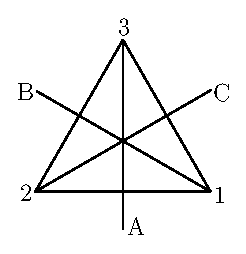
\includegraphics{images/lecture4/fig1.eps}

\smallskip

{\bf Equilateral Triangle}
\end{figure}

$D$ $\to$ clockwise rotation by $2\pi/3$ in the plane of the triangle.

$F$ $\to$ counter clockwise rotation by $2\pi/3$.
\begin{itemize}
\item Numbering of the corners destroys the symmetry $\to$ it is used here only for our understanding.

\item Axis does not rotate with the triangle $\to$ fixed in space.
\end{itemize}

For this we can create a group multiplication table.
\begin{center}
\begin{tabular}{>{$}c<{$}|>{$}c<{$}|>{$}c<{$}|>{$}c<{$}|>{$}c<{$}|>{$}c<{$}|>{$}c<{$}}
\hline 
 & E & A & B & C & D & F\\
\hline
E & E & A & B & C & D & F\\
A & A & E & D & F & B & C\\
B & B & F & E & D & C & A\\
C & C & D & F & E & A & B\\
D & D & C & A & B & F & E\\
F & F & B & C & A & E & D\\
\hline
\end{tabular}
\end{center}
\begin{align*}
&D \ {}_{2}\displaystyle{\mathop{\Delta}\limits^{3}}_{1}\to {}_{1}\displaystyle{\mathop{\Delta}\limits^{2}}_{3}\\
&D \ {}_{1}\displaystyle{\mathop{\Delta}\limits^{2}}_{3}\to {}_{3}\displaystyle{\mathop{\Delta}\limits^{1}}_{2}
\end{align*}
\begin{align*}
\therefore\quad DD &= F\\
                FF &= D\\
                FD &= DF=E
\end{align*}
$$
D=AB\neq BA=F\quad\text{Non-Abelian group.}
$$

The above table can be tested with the following matrices too
\begin{align*}
E &= \left(\begin{matrix} 1 & 0\\ 0 & 1\end{matrix}\right)\quad A=\left(\begin{matrix} 1 & 0 \\ 0 & -1\end{matrix}\right)\quad B=\left(\begin{matrix}-\dfrac{1}{2} & \dfrac{\sqrt{B}}{2}\\ \dfrac{\sqrt{3}}{2} & Y_{2}\end{matrix}\right)\\[5pt]
C &= \left(\begin{matrix} -\dfrac{1}{2} & -\dfrac{\sqrt{3}}{2}\\ -\dfrac{\sqrt{3}}{2} & \dfrac{1}{2}\end{matrix}\right)\quad D= \left(\begin{matrix} -\dfrac{1}{2} & \dfrac{\sqrt{3}}{2}\\ -\dfrac{\sqrt{3}}{2} & -\dfrac{1}{2}\end{matrix}\right)\quad F= \left(\begin{matrix}-\dfrac{1}{2} & -\dfrac{\sqrt{3}}{2}\\ \dfrac{\sqrt{3}}{2} & -\dfrac{1}{2}\end{matrix}\right)
\end{align*}
\end{example*}

\noindent
{\bf Isomorphic :} Two groups obeying same group multiplication table are called {\bf isomorphic}.

\noindent
{\bf Rearrangement Theorem :} In the sequence $EA_{k}$, $A_{2}A_{k}$, $A_{3}A_{k}\ldots A_{h}A_{k}$, each group element, $A_{i}$ occurs exactly once. The elements merely rearrange via group multiplication.

\begin{proof}
For any $A_{i}$, $A_{k}$ there exist an element $A_{r}=A_{i}A_{k}$. Since, the group contains {\bf inverses} and {\bf closed}. Again, $A_{r}A_{k}=A_{i}$. For this $A_{r}$, $A_{i}$ must appear at least once. But total no. of elements $=h$.

$\therefore$ \ There is no chance that any element will make more than one appearance.
\end{proof}

\noindent
{\bf Cyclic Group :} For any group element $X$, one can form the sequence
$$
X,X^{2},X^{3},\ldots,X^{n-1},X^{n}=E
$$

This is called period of $X$ since the sequence will repeat this period over and over if it extended. 

[Eventually one has to find the period since the group is finite]
$$
n\to \text{ order of } X
$$

The above sequence is called cyclic group of order $n$.
\begin{itemize}
\item If it is part of a larger group, it is called cyclic subgroup.

\item All cyclic groups are {\bf abelian group}.
\end{itemize}

In the example of triangle - the period of $D$ is $D$, $D^{2}=F$, $D^{3}=DF=E\Rightarrow n=3$, $D$, $F$, $E$ form a cyclic subgroup of the entire group of order $6$.

\noindent
{\bf Subgroups and Cosets Subgroup :} A part of the group containing unit element.

Let $S=E$, $S_{2}$, $S_{3},\ldots S_{g}$ is a subgroup of order $g$. Larger group has order $h$. Group = $g$.

If $X\in g$ but $x\not\in S$

Then, $EX$, $S_{2}X$, $S_{3}X,\ldots S_{g}X$ form {\bf right coset} $SX$ [If $X\in S$, then the $SX$ would be $S$ itself].

Left Coset : $XS$
\begin{itemize}
\item Cosets are not subgroup as it does not have identity element.

\item A coset has no element in common with the subgroup. 
\end{itemize}

\begin{proof}
If $X_{k}X=S_{l}$ a member of $S$.

Then $X=S^{-1}_{k}S_{l}$ will also be in $S$ [groups are closed]

Then $SX$ is not a coset it is $S$ itself.
\end{proof}

\begin{itemize}
\item Two right cosets of subgroup $S$ are identical or have no element in common.
\end{itemize}

\begin{proof}
Assume there is an element common in $SX$ and $SY$ which is $S_{k}X=S_{l}Y$

Then $XY^{-1}=S^{-1}_{k}S_{l}$ is in $S$

$\therefore \ SXY^{-1}=S$ post multiply by $Y$

We get \fbox{$SX=SY$}
\end{proof}

\begin{itemize}
\item Order of $g$ is $h$, which is integral multiple of the order of subgroup $g$. $\Rightarrow$ \fbox{$\dfrac{h}{g}=n$, $n$ integer}.
\end{itemize}

\begin{proof}
$h$ element of $g$ must appear in $S$ or in the cosets.

$\therefore$ Each element must be in one of the set
$$
S, \underbrace{SX_{1},SX_{2},SX_{3},\ldots,SX_{n}}_{\text{distinct cosets contain of element each}}
$$
$\therefore \ h=g\times n$.
\end{proof}

\begin{example*}
Triangle : $S=A$, $E$ order $=2=g$
\begin{alignat*}{2}
& SB = SD=B,D &~ \to~ & \text{identical cosets } \Rightarrow 6=2\times 3\\
& SF= C,F &~\to~ & \text{Distinct coset}.
\end{alignat*}
\end{example*}
\begin{itemize}
\item Order of any cyclic subgroup formed by the period of some group element must be a divisor of the order of the group.
\end{itemize}

\section*{Example Groups of Finite Order}

\begin{enumerate}
\item Group of order 1 : $E$

\item Group of order 2 : $A$, $A^{2}=E$ {\bf Abelian Group}

Reflection, Inversion, Interchange of two identical parties.

\item Group of order 3 : $A$, $A^{2}=B\neq E$, $A^{3}=E$

\item Group of order 4 : Two Possibilities
\begin{itemize}
\item $A$, $A^{2}$, $A^{3}$, $A^{4}=E$

\item Vierergruppe $(A,B,C,E)$ $\to$ rotational symmetry group of a rectangular solid.
\begin{figure}[H]
\centering
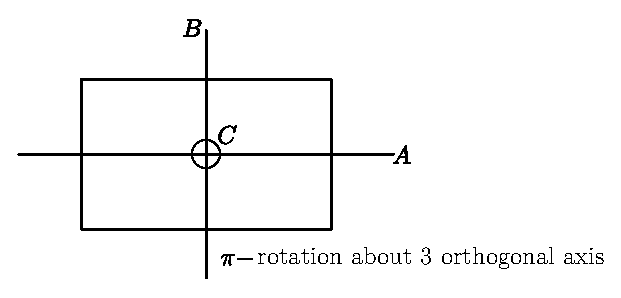
\includegraphics{images/lecture4/fig2.eps}
\end{figure}
\begin{center}
\textbf{Group multiplication table.}
\medskip

\begin{tabular}{>{$}c<{$}|>{$}c<{$}|>{$}c<{$}|>{$}c<{$}|>{$}c<{$}}
\hline
 & E & A & B & C\\
\hline
E & E & A & B & C\\
A & A & E & C & B\\
B & B & C & E & A\\
C & C & B & A & E\\
\hline
\end{tabular}
\end{center}
\end{itemize}

\item {\bf Groups of prime order :} They are cyclic abelian group otherwise {\bf the period of some element would have to appear as subgroup} whose order is a divisor of a prime number.

$\therefore$ \ There can be single groups of order $1,2,3,5,7,11,13\ldots$

\item {\bf Permutation Group :} (of factorial order)

One group of order $n$ can always be set up based on all permutations of $n$ distinguishable things.

E.g.
$$
\left(
\begin{matrix}
1 & 2 & 3 & 4 & \ldots & n\\
\alpha_{1} & \alpha_{2} & \alpha_{3} & \alpha_{4} & \ldots & \alpha_{n}
\end{matrix}
\right)
$$
$\alpha$'s are $1,2,3$ in some order.

Here item $i$ is shifted to the position $\alpha_{i}$
\end{enumerate}

\begin{example*}
For\quad \raisebox{-.5cm}{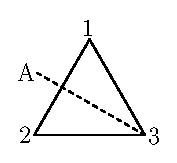
\includegraphics[scale=.7]{images/lecture4/fig3.eps}}
\begin{align*}
& E=\left(\begin{matrix} 1 & 2 & 3\\ 1 & 2 & 3\end{matrix}\right)\quad A=\left(\begin{matrix} 1 & 2 & 3\\ 2 & 1 & 3\end{matrix}\right)\quad B=\left(\begin{matrix} 1 & 2 & 3\\ 1 & 3 & 2\end{matrix}\right)\\[5pt]
& C=\left(\begin{matrix} 1 & 2 & 3\\ 3 & 2 & 1\end{matrix}\right)\quad D=\left(\begin{matrix} 1 & 2 & 3\\ 3 & 1 & 2\end{matrix}\right)\quad F=\left(\begin{matrix} 1 & 2 & 3\\ 2 & 3 & 1\end{matrix}\right)
\end{align*}

$A \to$ Reflection with respect of $A$; 1 \& 2 interchange, $3\to$ same.

$D\to$ Anti-clockwise rotation by $2\frac{\pi}{3}$.
\begin{figure}[H]
\centering
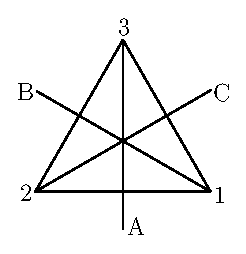
\includegraphics{images/lecture4/fig4.eps}
\end{figure}
Axis remains fixed in space.
\begin{figure}[H]
\centering
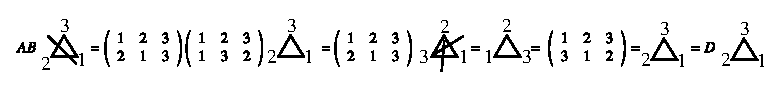
\includegraphics{images/lecture4/fig5.eps}
\end{figure}

Because of the identity of like particles, permutation of them leaves the Hamiltonian invariant.
\end{example*}

\section*{Conjugate Elements and Class Structure}

An element $B$ is conjugate to $A$ if
$$
B=XAX^{-1}\quad\text{or}\quad A=X^{-1}BX\quad X\in g
$$
These are {\bf reciprocal pairs.}
